\graphicspath{{./figures}}

\section{Ground Station Antenna}

The initial helical ground station antenna is shown in Figure \ref{fig:groundStationAntenna}. 2.5 mm stranded copper wire was used due to its flexibility and availability. A cardboad ground plane wrapped in aluminium foil was used due to its lightweight nature. Further, a strip of harder aluminium tin was connected to the wire for the matching strip. Tape was then used to provide an electrical connection. The strip was made over-sized for initial testing. A female panel-mounted SMA connector was then mounted using bolts, and the wire was attached to the protruding pin.

The coiled wire is supported by a central PVC pipe and wooden dowels for mechanical support. Markings on the pipe were used to dimension the antenna. The materials were sized to provide stability, but not exceed the maximum torque limitations of the motors. The final antenna weight was measured at xxx.

\begin{figure}[!htb]
  \centering
  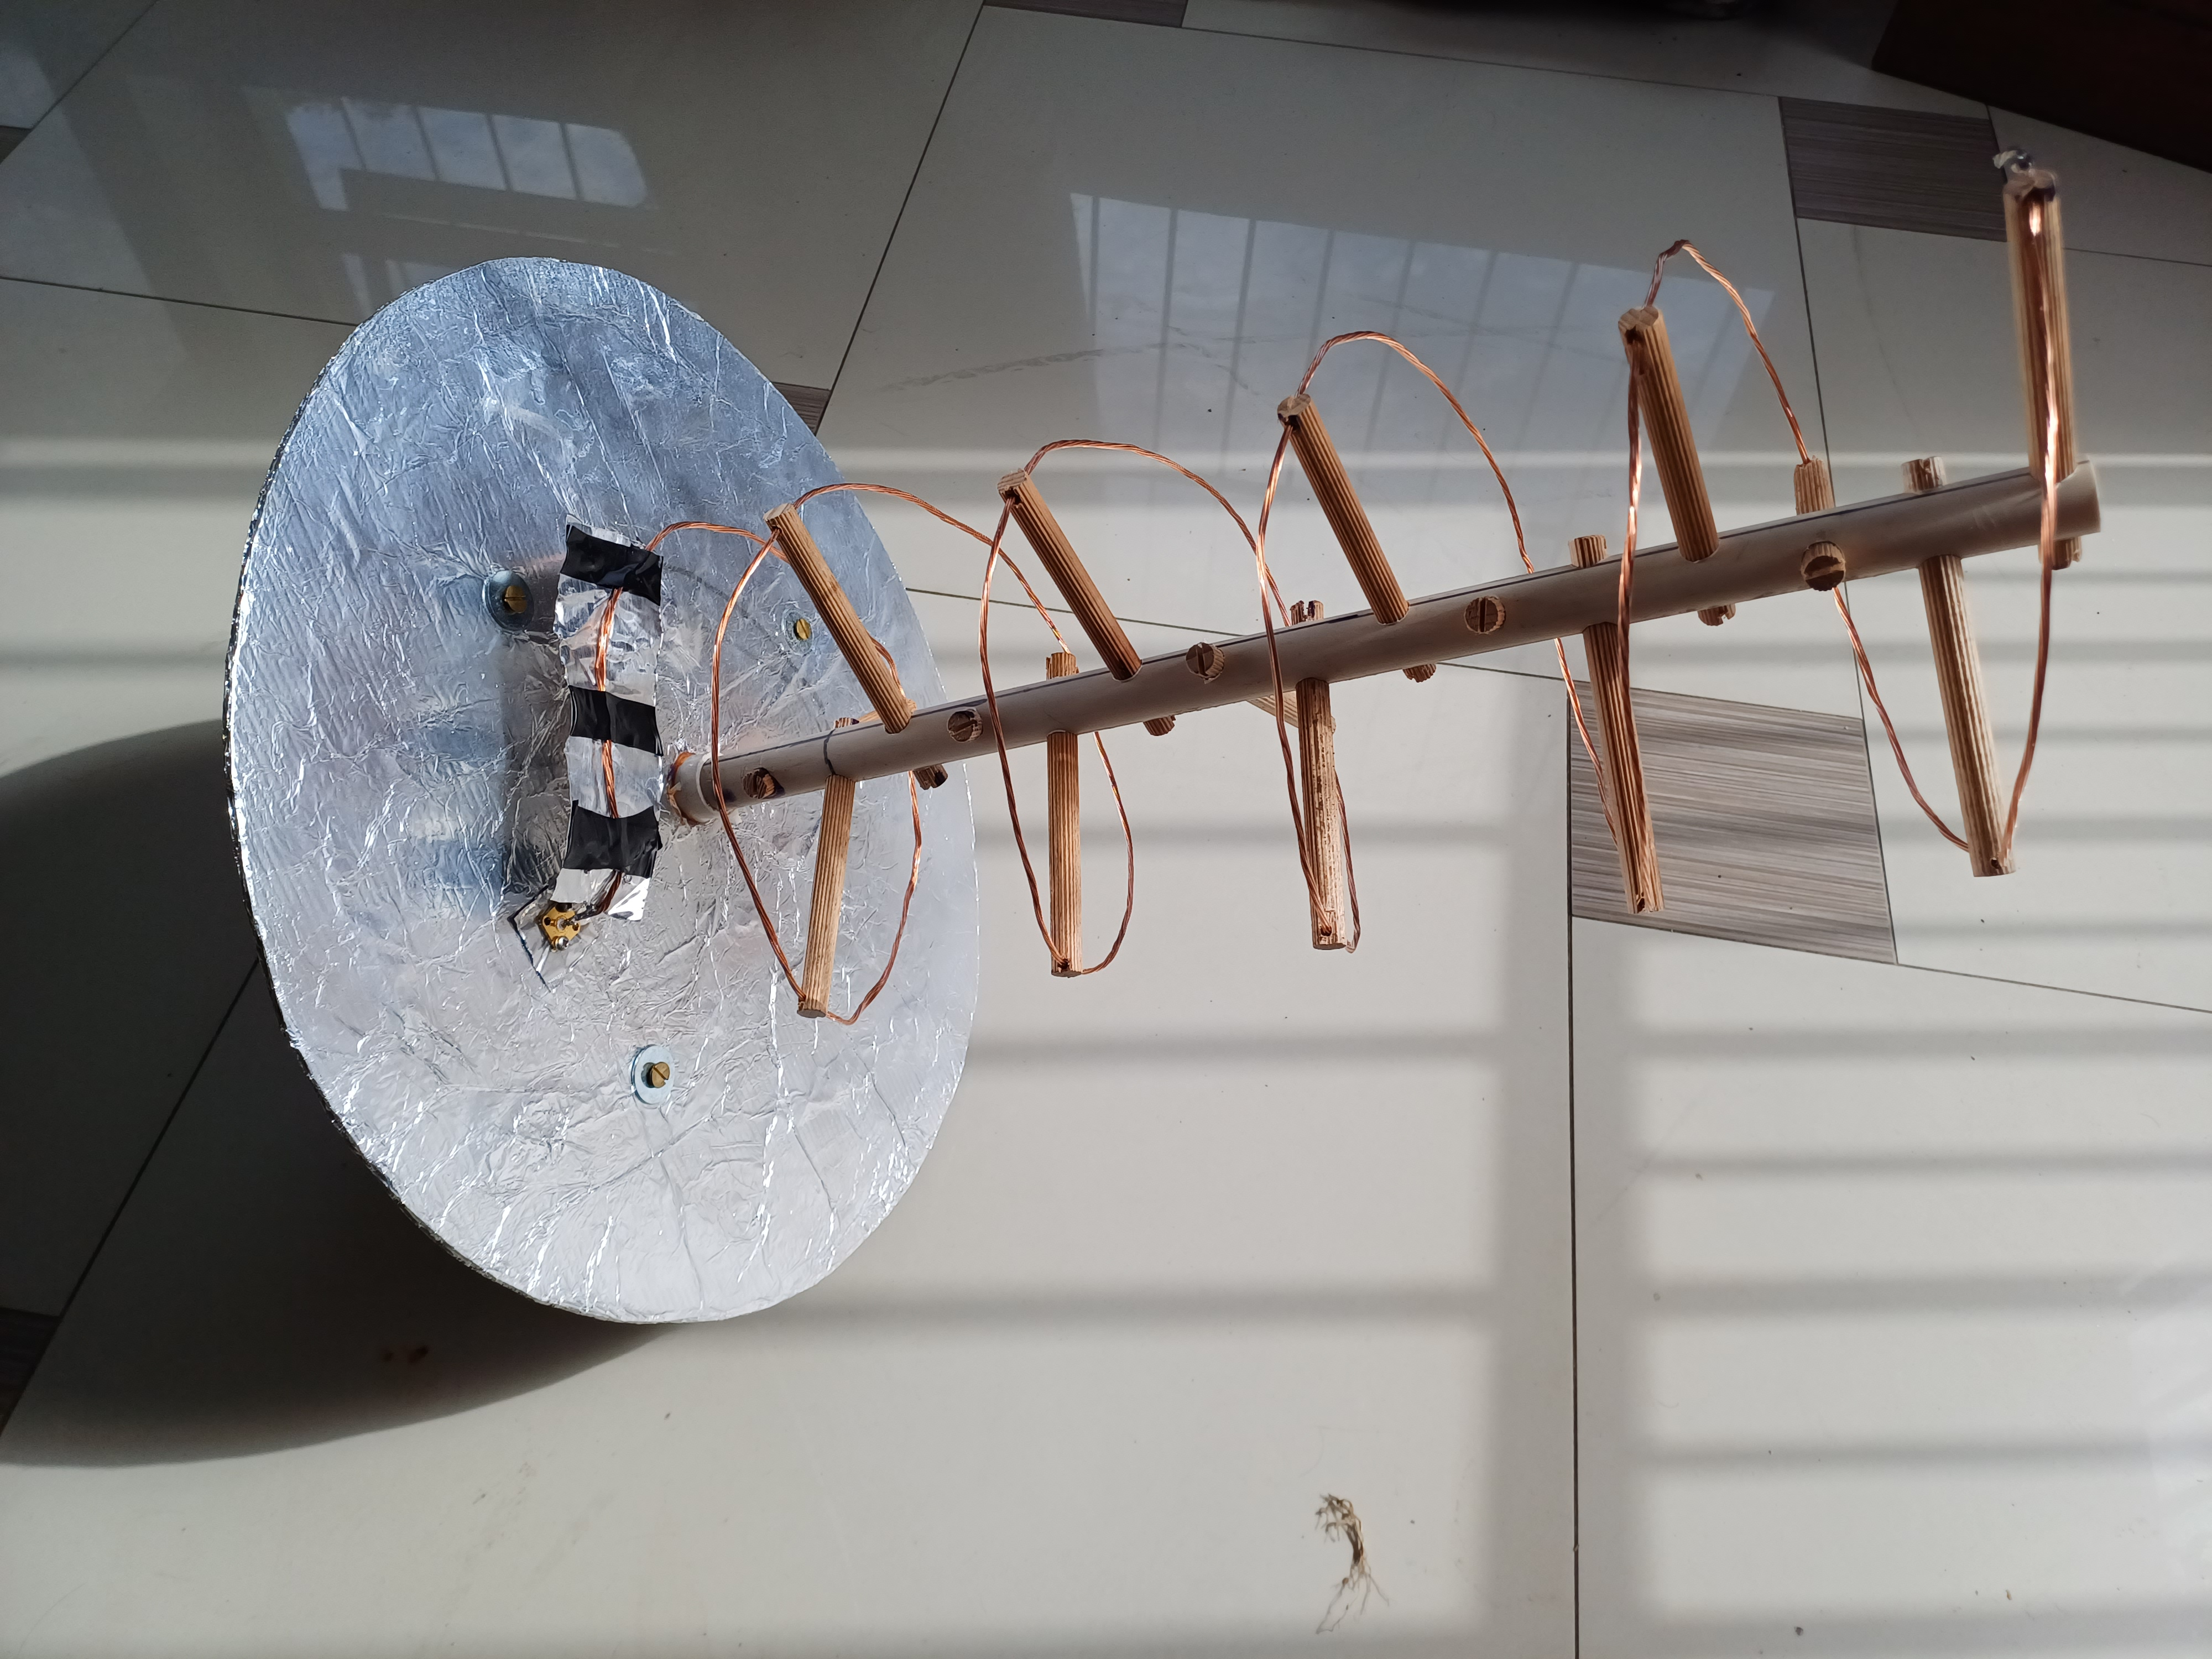
\includegraphics[width=0.6\textwidth]{groundStationAntenna}
  \caption{Ground Station Antenna Build}
  \label{fig:groundStationAntenna}
\end{figure}